% !TEX root = ../main.tex
\section{Метод Понтрягіна}
У випадку простого руху в $\R^n$ замість системи диференціальних рівнянь,
що описують рух переслідувача та утікача розглядалося
одне диференціальне рівняння, що описувало динаміку різниці їх положень.
\begin{definition}
    \emph{Лінійною диференціальною грою} називається гра з фазовим простором
    $\R^n$, що описується рівнянням
    \begin{gather}\label{lin_game}
        \begin{cases}
            \d{z}(t) = A z(t) - u(t) + v(t) \\
            z(0) = z_0 \\
            u \in U, \; v \in V
        \end{cases}
    \end{gather}
    де $A$ --- деяка стала матриця порядку $n\times n$, $U$ та $V$ --- опуклі компактні
    підмножини $\R^n$. Також задано матрицю $\pi$, що є матрицею проекції на ортогональне доповнення до термінальної множини.
\end{definition}
Ця гра відбувається таким чином: в кожний момент часу $t$ утікач $E$ знає параметри гри
$\l(A, U, V, z_0, \pi \r)$ та обирає своє керування $v(t) \in V$, повідомляючи про свій вибір
переслідувача $P$, який, в свою чергу, обирає керування $u(t) \in U$.
Якщо існує такий момент часу $T > 0$, коли переслідувач $P$ за будь-яких дій
утікача $E$ забезпечує виконання умови $\pi z(\tau) = 0$ для деякого
$\tau \in [0; T]$, то кажуть, що в переслідувач наздоганяє утікача.
Отримаємо умови, за яких це відбувається. Для цього треба ввести декілька нових означень.
\begin{definition}
    \emph{Сумою множин (за Мінковським)} $A$ і $B$ називається множина
    $C = A + B = \l\{ a + b : a \in A, b \in B\r\}$.
\end{definition}
\begin{definition}
    \emph{Різницею множин (за Мінковським)} $A$ і $B$ називається найбільша така множина
    $C = A \setdif B$, що $B + C \subset A$
\end{definition}
\begin{definition}
    \emph{Добутком} множини $A$ на число $\lambda \in \R$ називається множина
    $\lambda \cdot A = \l\{\lambda \cdot a : a \in A \r\}$.
\end{definition}
\begin{example}
    Нехай $B_{r}(a) = \l\{x \in \R^n : \norm{x - a} \leq r \r\}$ --- куля
    радіуса $r$ з центром в точці $a$. Для
    $r \in \R$ та $a \in \R^n$ має місце
    $r\cdot B_{1}(0) + \{a\} = B_{|r|}(a)$.
    Сумою двох куль $B_{r_1}(a_1)$ та $B_{r_2}(a_2)$ є множина
    \begin{gather*}
        M = B_{r_1}(a_1) + B_{r_2}(a_2) = \l\{ 
            x_1 + x_2 : \norm{x_1 - a_1} \leq r_1, \norm{x_2 - a_2} \leq r_2    
        \r\}
    \end{gather*}
    Для $x = x_1 + x_2 \in M$: $\norm{(x_1 + x_2) - (a_1 + a_2)} \leq \norm{x_1 - a_1} + \norm{x_2 - a_2} \leq r_1 + r_2$,
    тобто $M = B_{r_1 + r_2}(a_1 + a_2)$.
    \begin{center}
        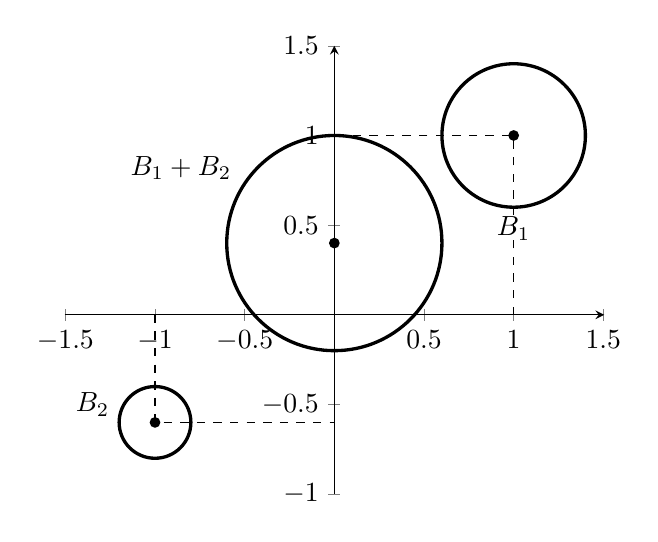
\begin{tikzpicture}
            \begin{axis}
                [axis lines = center,
                axis equal,
                trig format plots=rad,
                xmin=-1.5, xmax=1.5, ymin=-1, ymax=1.5,
                legend pos = outer north east]
                \draw [very thick] (1,1) circle (0.4);
                \draw [very thick] (-1,-0.6) circle (0.2);
                \draw [very thick] (0,0.4) circle(0.6);
                \node [below] at (1,0.6) {$B_1$};
                \node [left] at (-1.2,-0.5) {$B_2$};
                \node [above left] at (-0.52,0.7) {$B_1 + B_2$};
                \draw [dashed] (1,0) -- (1,1) -- (0,1);
                \draw [dashed] (-1,0) -- (-1,-0.6) -- (0,-0.6);
                \fill (1,1) circle (0.03);
                \fill (-1,-0.6) circle (0.03);
                \fill (0,0.4) circle (0.03);
            \end{axis}
        \end{tikzpicture}
    \end{center}
    
\end{example}
\begin{definition}
    Нехай $W(t)$ --- функція з дійсним аргументом, значеннями якої
    є компактні підмножини $\R^n$ (\emph{багатозначне відображення}).
    \emph{Інтегралом} за проміжком $[a;b]$ від неї називається множина
    $\intl_a^b W(t) dt$, яку можна розуміти в сенсі ріманової суми
    $\underset{n\to\infty}{\lim} \suml_{i=0}^n \Delta t_i\cdot W(t_i^*)$,
    де $\l\{\Delta t_i\r\}_{i=1}^n$ --- довжини відрізків, на які розбивається $[a;b]$, $t_i^* \in \Delta t_i$ ---
    деякі точки з цих відрізків, а сума розуміється в сенсі суми множин за Мінковським.
\end{definition}
\begin{example}\label{ball_intergral}
    Нехай $W(t) = B_t(0)$, $[a;b] = [0; T]$. Знайдемо 
    $\intl_0^T W(t) dt$.
    $\suml_{i=0}^n \Delta t_i\cdot W(t_i^*) = \suml_{i=0}^n \Delta t_i\cdot B_{t_i^*}(0) = 
    \suml_{i=0}^n B_{t_i^* \Delta t_i}(0) = B_{\suml_{i=0}^n t_i^* \Delta t_i} (0)$ --- це
    куля з центром в $0$ та радіусом $\suml_{i=0}^n t_i^* \Delta t_i$. Вираз для радіуса
    є інтегральною сумою для $\intl_0^t t dt = \frac{T^2}{2}$, тому
    $\intl_0^T B_t(0) dt = B_{\frac{T^2}{2}} (0)$.
\end{example}
Нехай у грі (\ref{lin_game}) виконуються дві умови:
\begin{enumerate}
    \item Для всіх $t>0$: $W(t) = \pi e^{At}U \setdif \pi e^{At}V \neq \varnothing$.
    \item Існує такий момент часу $T_0$, що $\pi e^{AT_0}z_0 \in \intl_0^T W(T_0 - s)ds$.
\end{enumerate}

Можна довести (див. \cite{4}), що в разі виконання цих умов переслідувач наздожене утікача.
Пояснення цього наводиться в \cite{3}. Розв'язок задачі Коші та його образ під дією $\pi$ у (\ref{lin_game}) мають вигляд
\begin{gather}
    z(t) = e^{A t} z_0 + \intl_0^t e^{A(t-s)} (- u(s) + v(s)) ds
\end{gather}
\begin{gather}\label{4_3}
    \pi z(t) =  \pi e^{A t} z_0 + \intl_0^t \pi e^{A(t-s)} (- u(s) + v(s)) ds
\end{gather}
За умовою 2 існує $w(T_0, s) \in W(T_0-s)$ такий, що $\pi e^{AT_0}z_0 = \intl_0^{T_0} w(T_0, s) ds$. Переслідувач має обирати своє керування
$\widehat{u}(s)$ як розв'язок рівняння
\begin{gather*}
    \pi e^{A (T_0-s)} u(s) - \pi e^{A (T_0-s)} v(s) = w(T_0, s) 
\end{gather*}
Існування розв'язку гарантується умовою 1. Якщо підставити знайдене $\widehat{u}(s)$ в (\ref{4_3}),
отримаємо 
$
    \pi z(T_0) = \pi e^{A T_0} z_0 - \intl_0^t w(T_0, s) ds = 0
$, що означає, що в момент $T_0$ переслідувач наздожене утікача.

В \cite{3} пропонується \emph{алгоритм застосування методу Понтрягіна:}
\begin{enumerate}
    \item Знайти множину $W(t) = \pi e^{At}U \setdif \pi e^{At}V$.
    \item Знайти множину $\Omega(t) = \intl_0^t W(s)ds$.
    \item Знайти $T_0$, для якого $\pi e^{A T_0} z_0 \in \Omega(T_0)$.
    \item Знайти функцію $w(t) \in W(t)$ таку, що $\pi e^{A T_0} z_0 = \intl_0^{T_0} w(s) ds$.
    \item Знайти керування $u(t)$ як розв'язок $\pi e^{A (T_0-s)} u(s) - \pi e^{A (T_0-s)} v(s) = w(T_0 - s) $ при заданому керуванні $v(t) \in V$.
    \item Знайти розв'язок задачі Коші $\d{z} = Az - u(t) + v(t), \; z(0) = z_0$ на відрізку $[0; T_0]$.
\end{enumerate}

\begin{example}[контрольний приклад Понтрягіна, \cite{4}]\label{ex_4_3}
    Нехай рух гравців в $\R^n$, $n\geq 2$, описується системою
    \begin{gather*}
        \begin{cases}
            \dd{x} + \alpha \d{x} = a, & \norm{a} \leq \rho \\
            \dd{y} + \beta \d{y} = b, & \norm{b} \leq \sigma
        \end{cases}
    \end{gather*}
    де $\alpha, \beta, \rho, \sigma$ --- додатні числа. Переслідувач наздоганяє утікача, якщо $x=y$.
    Ця системи описує рух точки одиничної маси під дією сили-керування з урахуванням тертя,
    що лінійно залежить від швидкості.
    Перейдемо до системи диференціальних рівнянь першого порядку за допомогою замін $z^1 = x - y$, $z^2 = \d{x}$, $z^3 = \d{y}$:
    \begin{gather*}
        \begin{cases}
            \d{z}^1 = z^2 - z^3 \\
            \d{z}^2 = -\alpha z^2 + a \\
            \d{z}^3 = -\beta z^3 + b
        \end{cases}
    \end{gather*}
    Керування $u$ та $v$ задаються формулами $u = (0, -a, 0)^T$, $v = (0, 0, b)^T$, тому
    $U = \l\{(0, -a, 0)^T : \norm{a} \leq \rho \r\}$, $V = \l\{(0, 0, b)^T : \norm{b} \leq \sigma \r\}$.
    Оператор $\pi$ задано як $\pi: (z^1, z^2, z^3)^T \mapsto (z^1, 0, 0)^T$, а матриця $A$
    дорівнює $\begin{pmatrix}
        0 & 1 & -1 \\
        0 & -\alpha & 0 \\
        0 & 0 & -\beta
    \end{pmatrix}$. Знайдемо $e^{A t}$ (за допомогою перетворення Лапласа):
    \begin{gather*}
        e^{At} = \Lap{(pI - A)^{-1}} \Leftrightarrow (pI - A)^{-1} = \LapInv{e^{At}} \\
        pI - A = \begin{pmatrix}
            p & -1 & 1 \\
            0 & p+\alpha & 0 \\
            0 & 0 & p + \beta \\
        \end{pmatrix} \\
        (pI - A)^{-1} = \frac{1}{p(p+\alpha)(p+\beta)}\begin{pmatrix}
            (p+\alpha)(p+\beta) & (p+\beta) & -(p+\alpha) \\
            0 & p(p+\beta) & 0 \\
            0 & 0 & p(p+\alpha)
        \end{pmatrix} = \\ =
        \begin{pmatrix}
            \frac{1}{p} & \frac{1}{p(p+\alpha)} & - \frac{1}{p(p+\beta)} \\
            0 & \frac{1}{p+\alpha} & 0 \\
            0 & 0 & \frac{1}{p+\beta}
        \end{pmatrix} \Rightarrow
        e^{At} = \begin{pmatrix}
            1 & \frac{1 - e^{-\alpha t}}{\alpha} & -\frac{1 - e^{-\beta t}}{\beta} \\
            0 & e^{-\alpha t} & 0 \\
            0 & 0 & e^{-\beta t}
        \end{pmatrix}
    \end{gather*}
    Тепер можна записати $\pi e^{At}(z^1, z^2, z^3) = z^1 + \frac{1 - e^{-\alpha t}}{\alpha} z^2 - \frac{1 - e^{-\beta t}}{\beta}z^3$, звідки
    \begin{gather*}
        \pi e^{At} U = \l\{\frac{1 - e^{-\alpha t}}{\alpha} \cdot (-a) : \norm{a} \leq \rho\r\} \\ 
        \pi e^{At} V = \l\{-\frac{1 - e^{-\beta t}}{\beta} \cdot b : \norm{b} \leq \sigma\r\}
    \end{gather*}
    Отже, $\pi e^{At} U$ --- куля з радіусом $\frac{1 - e^{-\alpha t}}{\alpha}\rho$ і центром в нулі,
    а $\pi e^{At} V$ --- куля з радіусом $\frac{1 - e^{-\beta t}}{\beta}\sigma$ і центром в нулі, тому
    $W(t) = \pi e^{At}U \setdif \pi e^{At}V$ --- куля з радіусом 
    $\frac{1 - e^{-\alpha t}}{\alpha}\rho - \frac{1 - e^{-\beta t}}{\beta}\sigma$ і центром теж в нулі.
    Радіус $W(t)$ буде додатнім при $\rho > \sigma$ та $\frac{\rho}{\alpha} > \frac{\sigma}{\beta}$.
    Аналогічно прикладу \ref{ball_intergral}, $\Omega(t) = \intl_0^t W(s) ds$ буде кулею
    з радіусом
    \begin{gather*}
        \intl_0^t \left(\frac{1 - e^{-\alpha st}}{\alpha}\rho - \frac{1 - e^{-\beta s}}{\beta} \sigma\right) ds = 
        \rho \intl_0^t \frac{1 - e^{-\alpha st}}{\alpha} ds - \sigma \intl_0^t \frac{1 - e^{-\beta s}}{\beta} ds =
    \end{gather*}
    \begin{gather*}
        = \frac{\rho}{\alpha^2}\l(\alpha t + e^{-\alpha t} - 1\r) - 
        \frac{\sigma}{\beta^2}\l(\beta t + e^{-\beta t} - 1\r) = r(t)
    \end{gather*}
    Далі необхідно знайти таке (найменше) значення $T_0$, для якого точка $\pi e^{A T_0}(z^1_0, z^2_0, z^3_0)$ належить
    $\Omega(T_0)$. З геометричних міркувань це буде найменший корінь рівняння
    \begin{gather*}
        \frac{\rho}{\alpha^2}\l(\alpha t + e^{-\alpha t} - 1\r) - 
        \frac{\sigma}{\beta^2}\l(\beta t + e^{-\beta t} - 1\r) = \norm{\pi e^{A t} z_0}
    \end{gather*}
    
    Наступний крок будемо проводити на конкретному прикладі. Нехай гра відбувається на площині з 
    $\alpha=1$, $\beta=2$, $\rho=2$, $\sigma=1$ та
    початковими умовами $x(0) = \begin{pmatrix}
        3 \\ 2
    \end{pmatrix}, \d{x}(0) = \begin{pmatrix}
        1 \\ 1
    \end{pmatrix}, y(0) = \begin{pmatrix}
        1 \\ 0
    \end{pmatrix}, \d{y}(0) = \begin{pmatrix}
        0 \\ 1
    \end{pmatrix}$. Чисельно можна знайти значення $T_0 \approx 3.715$.
    \begin{center}
        % This file was created by tikzplotlib v0.9.8.
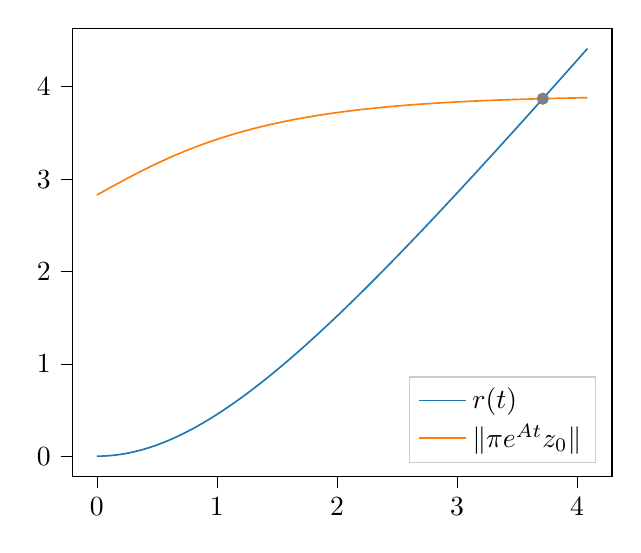
\begin{tikzpicture}

\definecolor{color0}{rgb}{0.12156862745098,0.466666666666667,0.705882352941177}
\definecolor{color1}{rgb}{1,0.498039215686275,0.0549019607843137}

\begin{axis}[
legend cell align={left},
legend style={
  fill opacity=0.8,
  draw opacity=1,
  text opacity=1,
  at={(0.97,0.03)},
  anchor=south east,
  draw=white!80!black
},
tick align=outside,
tick pos=left,
x grid style={white!69.0196078431373!black},
xmin=-0.204323093744256, xmax=4.29078496862938,
xtick style={color=black},
y grid style={white!69.0196078431373!black},
ymin=-0.220660969615349, ymax=4.63388036192233,
ytick style={color=black}
]
\addplot [draw=none, draw=gray, fill=gray, forget plot, mark=*]
table{%
x  y
3.7149653408046555 3.871012274588237
};
\addplot [semithick, color0]
table {%
0 0
0.0412773926756073 0.000851675551739262
0.0825547853512146 0.00340396133088938
0.123832178026822 0.00764899720016565
0.165109570702429 0.0135744146071706
0.206386963378036 0.021163901319297
0.247664356053644 0.0303977130192026
0.288941748729251 0.0412531363108558
0.330219141404858 0.0537049073118955
0.371496534080466 0.0677255896639957
0.412773926756073 0.0832859154766872
0.45405131943168 0.100355092429385
0.495328712107287 0.118901079989231
0.536606104782895 0.138890837456842
0.577883497458502 0.160290546326417
0.619160890134109 0.183065809239396
0.660438282809717 0.20718182762035
0.701715675485324 0.232603559908876
0.742993068160931 0.259295862140481
0.784270460836539 0.287223612481875
0.825547853512146 0.316351821190482
0.866825246187753 0.346645727343524
0.90810263886336 0.378070883567689
0.949380031538968 0.410593229895515
0.990657424214575 0.444179157778245
1.03193481689018 0.478795565196554
1.07321220956579 0.514409903729416
1.1144896022414 0.550990218366914
1.155766994917 0.588505180784594
1.19704438759261 0.626924116734254
1.23832178026822 0.666217028148695
1.27959917294383 0.706354610505276
1.32087656561943 0.747308265944848
1.36215395829504 0.789050112598411
1.40343135097065 0.831552990533316
1.44470874364626 0.874790464693667
1.48598613632186 0.918736825175607
1.52726352899747 0.963367085147013
1.56854092167308 1.00865697669263
1.60981831434868 1.05458294483956
1.65109570702429 1.10112213999425
1.6923730996999 1.14825240900014
1.73365049237551 1.19595228500534
1.77492788505111 1.24420097631142
1.81620527772672 1.29297835435761
1.85748267040233 1.34226494097973
1.89876006307794 1.3920418950691
1.94003745575354 1.44229099874407
1.98131484842915 1.49299464313515
2.02259224110476 1.54413581387452
2.06386963378036 1.59569807637061
2.10514702645597 1.64766556094006
2.14642441913158 1.70002294786138
2.18770181180719 1.75275545240719
2.22897920448279 1.80584880990557
2.2702565971584 1.85928926087503
2.31153398983401 1.91306353627204
2.35281138250962 1.9671588428854
2.39408877518522 2.02156284890709
2.43536616786083 2.07626366970525
2.47664356053644 2.13124985382142
2.51792095321204 2.1865103692107
2.55919834588765 2.24203458974067
2.60047573856326 2.29781228196219
2.64175313123887 2.35383359216281
2.68303052391447 2.41008903371129
2.72430791659008 2.46656947469998
2.76558530926569 2.52326612588994
2.8068627019413 2.58017052896202
2.8481400946169 2.63727454507615
2.88941748729251 2.69457034373945
2.93069487996812 2.7520503919828
2.97197227264372 2.80970744384485
3.01324966531933 2.86753453016111
3.05452705799494 2.92552494865546
3.09580445067055 2.98367225433055
3.13708184334615 3.04197025015309
3.17835923602176 3.10041297802949
3.21963662869737 3.15899471006699
3.26091402137298 3.21770994011503
3.30219141404858 3.27655337558126
3.34346880672419 3.33551992951656
3.3847461993998 3.39460471296288
3.4260235920754 3.45380302755809
3.46730098475101 3.51311035839132
3.50857837742662 3.57252236710275
3.54985577010223 3.63203488522127
3.59113316277783 3.69164390773383
3.63241055545344 3.75134558688004
3.67368794812905 3.81113622616557
3.71496534080466 3.87101227458824
3.75624273348026 3.93097032107035
3.79752012615587 3.99100708909118
3.83879751883148 4.05111943151347
3.88007491150708 4.11130432559795
3.92135230418269 4.17155886819989
3.9626296968583 4.23188027114197
4.00390708953391 4.29226585675761
4.04518448220951 4.35271305359942
4.08646187488512 4.41321939230698
};
\addlegendentry{$r(t)$}
\addplot [semithick, color1]
table {%
0 2.82842712474619
0.0412773926756073 2.85773589965896
0.0825547853512146 2.88717896014367
0.123832178026822 2.91661288129743
0.165109570702429 2.94591661713905
0.206386963378036 2.9749883778964
0.247664356053644 3.00374293894893
0.288941748729251 3.03210932626525
0.330219141404858 3.06002882791448
0.371496534080466 3.08745328651118
0.412773926756073 3.11434363279201
0.45405131943168 3.14066862562369
0.495328712107287 3.16640376844449
0.536606104782895 3.19153037637054
0.577883497458502 3.21603477193383
0.619160890134109 3.2399075906765
0.660438282809717 3.26314318063888
0.701715675485324 3.28573908219011
0.742993068160931 3.30769557670555
0.784270460836539 3.32901529434074
0.825547853512146 3.34970287262879
0.866825246187753 3.36976465887628
0.90810263886336 3.38920845038574
0.949380031538968 3.40804326742015
0.990657424214575 3.42627915457361
1.03193481689018 3.44392700684284
1.07321220956579 3.46099841722672
1.1144896022414 3.47750554313052
1.155766994917 3.49346098923186
1.19704438759261 3.50887770478715
1.23832178026822 3.52376889363096
1.27959917294383 3.53814793535269
1.32087656561943 3.55202831633319
1.36215395829504 3.56542356949292
1.40343135097065 3.57834722174821
1.44470874364626 3.59081274829621
1.48598613632186 3.6028335329564
1.52726352899747 3.61442283388869
1.56854092167308 3.62559375408822
1.60981831434868 3.6363592161262
1.65109570702429 3.64673194066661
1.6923730996999 3.6567244283414
1.73365049237551 3.66634894461273
1.77492788505111 3.67561750729147
1.81620527772672 3.68454187641684
1.85748267040233 3.69313354623337
1.89876006307794 3.7014037390292
1.94003745575354 3.70936340062458
1.98131484842915 3.71702319732106
2.02259224110476 3.72439351414148
2.06386963378036 3.73148445420832
2.10514702645597 3.73830583912348
2.14642441913158 3.74486721022637
2.18770181180719 3.75117783061985
2.22897920448279 3.75724668786463
2.2702565971584 3.7630824972529
2.31153398983401 3.76869370558097
2.35281138250962 3.77408849534897
2.39408877518522 3.77927478932283
2.43536616786083 3.78426025540077
2.47664356053644 3.78905231173211
2.51792095321204 3.79365813204203
2.55919834588765 3.79808465112057
2.60047573856326 3.80233857043875
2.64175313123887 3.80642636385863
2.68303052391447 3.81035428340783
2.72430791659008 3.81412836509229
2.76558530926569 3.81775443472399
2.8068627019413 3.82123811374324
2.8481400946169 3.82458482501725
2.88941748729251 3.82779979859931
2.93069487996812 3.83088807743455
2.97197227264372 3.83385452300023
3.01324966531933 3.83670382087017
3.05452705799494 3.83944048619426
3.09580445067055 3.84206886908544
3.13708184334615 3.84459315990761
3.17835923602176 3.84701739445928
3.21963662869737 3.84934545904819
3.26091402137298 3.85158109545372
3.30219141404858 3.85372790577398
3.34346880672419 3.85578935715574
3.3847461993998 3.85776878640549
3.4260235920754 3.85966940448096
3.46730098475101 3.86149430086243
3.50857837742662 3.86324644780397
3.54985577010223 3.86492870446503
3.59113316277783 3.86654382092287
3.63241055545344 3.86809444206721
3.67368794812905 3.86958311137803
3.71496534080466 3.87101227458824
3.75624273348026 3.87238428323279
3.79752012615587 3.87370139808624
3.83879751883148 3.87496579249052
3.88007491150708 3.87617955557531
3.92135230418269 3.877344695373
3.9626296968583 3.8784631418307
4.00390708953391 3.87953674972151
4.04518448220951 3.88056730145759
4.08646187488512 3.88155650980735
};
\addlegendentry{$\Vert\pi e^{At} z_0\Vert$}
\end{axis}

\end{tikzpicture}

    \end{center}
\end{example}
\begin{example}
    Розглянемо тепер гру з простим рухом:
    \begin{gather*}
        \begin{cases}
            \d{x} = u, & \norm{u} \leq \alpha \\
            \d{y} = v, & \norm{v} \leq \beta 
        \end{cases}
    \end{gather*}
    Зробимо заміну $z = x - y$: $\d{z} = u - v = -(-u) + (-v)$.
    переслідування закінчується, коли $z = x - y = 0$.
    В такому випадку оператор $\pi$ є тотожнім, матриця $A$ --- нульовою,
    тому й композиція $\pi e^{At} = I$ --- теж тотожній оператор.
    $U = B_{\alpha}(0)$, $V = B_{\beta}(0)$ --- кулі з центрами в $0$ та з радіусами
    $\alpha$ та $\beta$ відповідно. Таким чином, $W(t) = 
    \pi e^{At} U \setdif \pi e^{A t} V = U \setdif V = B_{\alpha - \beta}(0)$,
    при $\alpha \geq \beta$ ця множина є непорожньою.
    $\Omega(t) = \intl_0^t W(s)ds = B_{t(\alpha - \beta)}(0)$, тому
    \begin{gather*}
        \pi e^{AT_0} z_0 \in \Omega(T_0) \Leftrightarrow z_0 \in B_{T_0(\alpha - \beta)}(0) \Leftrightarrow
        \norm{z_0} = T_0(\alpha - \beta) \Leftrightarrow T_0 = \frac{\norm{z_0}}{\alpha - \beta}
    \end{gather*}
    Зауважимо, що такий само час було отримано у \ref{sec_3_2} іншими міркуваннями.
    Тепер знайдемо $w(t) \in W(t)$, для якої $\pi e^{A T_0} z_0 = \intl_0^{T_0} w(s)ds$:
    \begin{gather*}
        \pi e^{A T_0} z_0 = z_0 = \intl_0^{\frac{\norm{z_0}}{\alpha - \beta}} w(s) ds \Rightarrow
        w(s) \equiv (\alpha - \beta)\cdot \frac{z_0}{\norm{z_0}}
    \end{gather*}
    Для заданого керування утікача $v(t)$ знайдемо керування переслідувача $u(t)$:
    \begin{gather*}
        \pi e^{A (T_0-s)} u(s) - \pi e^{A (T_0-s)} v(s) = w(T_0 - s) \\
        u(s) - v(s) = (\alpha - \beta)\cdot \frac{z_0}{\norm{z_0}} \Leftrightarrow
        u(s) = v(s) + (\alpha - \beta)\cdot \frac{z_0}{\norm{z_0}}
    \end{gather*}
    Таким чином, можемо розв'язати задачу Коші
    \begin{gather*}
        \begin{cases}
            \d{z} = -u + v = (\beta - \alpha)\cdot \frac{z_0}{\norm{z_0}} \\
            z(0) = z_0
        \end{cases} \Rightarrow
        z(t) = (\beta - \alpha)\cdot \frac{z_0}{\norm{z_0}} t + z_0 \Leftrightarrow \\ \Leftrightarrow
        x(t) - y(t) = (\beta - \alpha)\cdot \frac{x_0 - y_0}{\norm{x_0 - y_0}} t + (x_0 - y_0)
    \end{gather*}
\end{example}

\section{Метод розв'язуючих функцій}
Цей метод належить А.О. Чикрію та детально досліджений у \cite{6}.
Розглядається не просто лінійна диференціальна гра виду \ref{lin_game}, а більш загальна
\emph{квазілінійна} гра виду 
\begin{gather}\label{qlin_game}
    \begin{cases}
        \d{z} = A z + \vf(u, v) \\
        z(0) = z_0 \\
        z \in \R^n, u \in U, v \in V
    \end{cases}
\end{gather}
де $\vf(u, v) : U\times V \to \R^n$ --- неперервна за обома змінними функція.
\begin{remark}
    У випадку $\vf(u,v) = -u + v$ отримуємо лінійну гру (\ref{lin_game}).
\end{remark}
Термінальна множина має вид $M^* = M^0 + M$, де
$M^0$ --- деякий лінійний підпростір $\R^n$, а $M$ --- компактна підмножина ортогонального доповнення $M^0$,
$\pi$ --- проектор на $(M^0)^\perp$.

Нехай $\vf(U, v) = \l\{\vf(u,v) : u \in U\r\}$ для фіксованої $v \in V$,
$W(t, v) = \pi e^{At} \vf(U, v)$,
$W(t) = \bigcap\limits_{v \in V} W(t, v), t\geq 0$. 
\begin{remark}
    У випадку $\vf(u,v) = -u + v$ $W(t) = \pi e^{At}U \setdif \pi e^{At} V$.
\end{remark}

Вводяться позначення:
\begin{gather*}
    \gamma(t) \in W(t) \text{ --- вимірна функція} \\
    \xi(t, z, \gamma(\cdot)) = \pi e^{A t} + \intl_0^t \gamma(\tau) d\tau \\
    \alpha(t, \tau, z, v, \gamma(\cdot)) = \\ = \sup\l\{ 
        \alpha \geq 0 : \l[ W(t-\tau, v) - \gamma(t-\tau)\r] \cap \alpha
        \l[M - \xi(t, z, \gamma(\cdot))\r] \neq \varnothing
    \r\} \\
    T(z, \gamma(\cdot) = \inf \l\{ 
        t\geq 0: \intl_0^t \underset{v\in V}{\inf} \alpha(t, \tau, z, v, \gamma(\cdot)) d\tau \geq 1
    \r\}
\end{gather*}

\begin{definition}
    $\alpha(t, \tau, z, v, \gamma(\cdot))$ називається \emph{розв'язуючою функцією}.  
\end{definition}

У \cite{6} доведено наступне: якщо $W(t) \neq \varnothing$ для всіх $t\geq 0$,
$M$ --- опукла множина, $T(z_0, \gamma_0(\cdot)) < +\infty$ для деякого початкового положення
$z_0$ та деякої $\gamma^0(\cdot)$, то за час $T(z_0, \gamma_0(\cdot))$ гравці потрапляють у термінальну множину.

Також у \cite{6} доведено, що якщо гра (\ref{qlin_game}) є лінійною,
$W(t) = \pi e^{At}U \setdif \pi e^{At} V \neq \varnothing$, існує неперервна 
$r(t): [0; +\infty) \to [0; +\infty)$ та число $l \geq 0$ такі, що
$\pi e^{A t}U = r(t) S$, $M = l S$, де $S$ --- одинична куля в $(M^0)^\perp$ з центром в нулі, то
при $\xi(t, z, \gamma(\cdot)) \notin l S$, розв'язуюча функція $\alpha$ може бути знайдена як найбільший додатний корінь квадратного рівняння
\begin{gather}\label{lin_res_func}
    \norm{\pi e^{a(t-\tau)}v + \gamma(t-\tau) - \alpha \cdot \xi(t, z, \gamma(\cdot))} = r(t-\tau) + \alpha l
\end{gather}

\begin{example}[контрольний приклад Понтрягіна, \cite{6}]\label{ex_4_5}
    Як у прикладі \ref{ex_4_3}, одразу перейдемо від системи
    \begin{gather*}
        \begin{cases}
            \dd{x} + \alpha \d{x} = \rho u, & \norm{a} \leq 1 \\
            \dd{y} + \beta \d{y} = \sigma v, & \norm{b} \leq 1
        \end{cases}
    \end{gather*}
    до системи з $z_1 = x - y$, $z_2 = \d{x}$, $z_3 = \d{y}$:
    \begin{gather*}
        \begin{cases}
            \d{z}_1 = z_2 - z_3 \\
            \d{z}_2 = -\alpha z_2 + \rho u \\
            \d{z}_3 = -\beta z_3 + \sigma v
        \end{cases}
    \end{gather*}
    Термінальна множина $M^* = \l\{z: z_1 = 0 \r\} = M^0 + \{0\}$, ортогональне доповнення
    $(M^0)^\perp =\l\{z: z_2 = z_3 = 0 \r\}$, тому $\pi = \begin{pmatrix}
        I & 0 & 0 \\
        0 & 0 & 0 \\
        0 & 0 & 0
    \end{pmatrix}$, де $I$ та $0$ --- тотожній та нульовий оператор відповідно.
    Оскільки у вихідній системі рівнянь $x, y \in \R^n$, то $z \in \R^{3n}$,
    то $\pi : \R^{3n} \to (M^0)^\perp$. Матриця системи
    $A = \begin{pmatrix}
        0 & E & -E \\
        0 & -\alpha E & 0 \\
        0 & 0 & -\beta E
    \end{pmatrix}$,
    $
    U = \l\{ \begin{pmatrix}0 \\ \rho u \\ 0 \end{pmatrix} : \norm{u} \leq 1\r\}
    $,
    $
    V = \l\{ \begin{pmatrix}0 \\ 0 \\ \sigma v \end{pmatrix} : \norm{v} \leq 1\r\}
    $.
    Аналогічно прикладу \ref{ex_4_3},
    \begin{gather*}
        \pi e^{At} U = \frac{1 - e^{-\alpha t}}{\alpha} \rho S, \;
        \pi e^{At} V = \frac{1 - e^{-\beta t}}{\beta} \sigma S \\
        W(t) = \l(\frac{1 - e^{-\alpha t}}{\alpha} \rho - \frac{1 - e^{-\beta t}}{\beta} \sigma\r) S = \omega(t) S
    \end{gather*}
    Радіус цієї кулі невід'ємний при $\rho \geq \sigma$ та $\frac{\rho}{\alpha} \geq \frac{\sigma}{\beta}$.
    Поклавши $\gamma(t) = 0$, отримаємо
    $\xi(t, z, 0) = z_1 + \frac{1 - e^{-\alpha t}}{\alpha} z_2 - \frac{1 - e^{-\beta t}}{\beta}z_3$.
    Ця задача задовольняє всі умови для пошуку розв'язуючої функції через (\ref{lin_res_func}):
    \begin{gather*}
        \norm{\frac{1 - e^{-\beta t}}{\beta} \sigma v - \alpha \cdot \xi(t, z, 0)} = \frac{1 - e^{-\alpha t}}{\alpha} \rho
    \end{gather*}
    У \cite{6} показується, що 
    \begin{gather*}
        \underset{\norm{v}\leq 1}{\min}{\alpha(t, \tau, z, v, 0)} = \frac{\omega(t-\tau)}{\norm{\xi(t, z, 0)}}
    \end{gather*}
    і мінімум досягається при $v = -\frac{\xi(t, z, 0)}{\norm{\xi(t, z, 0)}}$, а час, коли переслідувач наздожене утікача, визначається як
    \begin{gather*}
        T(z, 0) = \min \l\{ t\geq 0 : \intl_0^t \frac{\omega(t-\tau)}{\norm{\xi(t, z, 0)}} d\tau = 1 \r\}
    \end{gather*}
    або ж як найменший додатний корінь рівняння
    \begin{gather*}
        \norm{\xi(t, z, 0)} = \intl_0^t \l(\frac{1 - e^{-\alpha \tau}}{\alpha} \rho - \frac{1 - e^{-\beta \tau}}{\beta} \sigma\r) d\tau
    \end{gather*}
    
    Розглянемо тепер конкретний приклад. Нехай ця гра відбувається на площині з 
    $\alpha=1$, $\beta=2$, $\rho=2$, $\sigma=1$ та
    початковими умовами $x(0) = \begin{pmatrix}
        3 \\ 2
    \end{pmatrix}, \d{x}(0) = \begin{pmatrix}
        1 \\ 1
    \end{pmatrix}, y(0) = \begin{pmatrix}
        1 \\ 0
    \end{pmatrix}, \d{y}(0) = \begin{pmatrix}
        0 \\ 1
    \end{pmatrix}$.
    Чисельно можна знайти значення $T_0 \approx 3.715$.
    \begin{center}
        % This file was created by tikzplotlib v0.9.8.
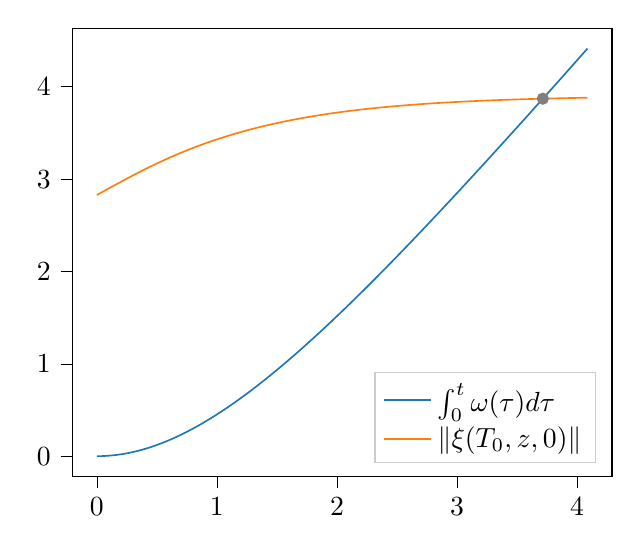
\begin{tikzpicture}

\definecolor{color0}{rgb}{0.12156862745098,0.466666666666667,0.705882352941177}
\definecolor{color1}{rgb}{1,0.498039215686275,0.0549019607843137}

\begin{axis}[
legend cell align={left},
legend style={
  fill opacity=0.8,
  draw opacity=1,
  text opacity=1,
  at={(0.97,0.03)},
  anchor=south east,
  draw=white!80!black
},
tick align=outside,
tick pos=left,
x grid style={white!69.0196078431373!black},
xmin=-0.204323093744256, xmax=4.29078496862938,
xtick style={color=black},
y grid style={white!69.0196078431373!black},
ymin=-0.220660969615349, ymax=4.63388036192233,
ytick style={color=black}
]
\addplot [draw=none, draw=gray, fill=gray, forget plot, mark=*]
table{%
x  y
3.7149653408046555 3.871012274588237
};
\addplot [semithick, color0]
table {%
0 0
0.0412773926756073 0.000851675551738981
0.0825547853512146 0.0034039613308894
0.123832178026822 0.00764899720016568
0.165109570702429 0.0135744146071706
0.206386963378036 0.021163901319297
0.247664356053644 0.0303977130192027
0.288941748729251 0.041253136310856
0.330219141404858 0.0537049073118953
0.371496534080466 0.0677255896639959
0.412773926756073 0.0832859154766874
0.45405131943168 0.100355092429385
0.495328712107288 0.118901079989231
0.536606104782895 0.138890837456842
0.577883497458502 0.160290546326418
0.619160890134109 0.183065809239396
0.660438282809717 0.20718182762035
0.701715675485324 0.232603559908876
0.742993068160931 0.259295862140481
0.784270460836539 0.287223612481875
0.825547853512146 0.316351821190482
0.866825246187753 0.346645727343524
0.908102638863361 0.378070883567689
0.949380031538968 0.410593229895515
0.990657424214575 0.444179157778245
1.03193481689018 0.478795565196554
1.07321220956579 0.514409903729416
1.1144896022414 0.550990218366914
1.155766994917 0.588505180784594
1.19704438759261 0.626924116734254
1.23832178026822 0.666217028148695
1.27959917294383 0.706354610505276
1.32087656561943 0.747308265944848
1.36215395829504 0.789050112598411
1.40343135097065 0.831552990533316
1.44470874364626 0.874790464693667
1.48598613632186 0.918736825175607
1.52726352899747 0.963367085147014
1.56854092167308 1.00865697669263
1.60981831434868 1.05458294483956
1.65109570702429 1.10112213999425
1.6923730996999 1.14825240900014
1.73365049237551 1.19595228500534
1.77492788505111 1.24420097631142
1.81620527772672 1.29297835435761
1.85748267040233 1.34226494097973
1.89876006307794 1.3920418950691
1.94003745575354 1.44229099874407
1.98131484842915 1.49299464313515
2.02259224110476 1.54413581387452
2.06386963378036 1.59569807637061
2.10514702645597 1.64766556094006
2.14642441913158 1.70002294786138
2.18770181180719 1.75275545240719
2.22897920448279 1.80584880990557
2.2702565971584 1.85928926087503
2.31153398983401 1.91306353627204
2.35281138250962 1.9671588428854
2.39408877518522 2.02156284890709
2.43536616786083 2.07626366970525
2.47664356053644 2.13124985382142
2.51792095321205 2.1865103692107
2.55919834588765 2.24203458974067
2.60047573856326 2.2978122819622
2.64175313123887 2.35383359216281
2.68303052391447 2.41008903371129
2.72430791659008 2.46656947469998
2.76558530926569 2.52326612588994
2.8068627019413 2.58017052896202
2.8481400946169 2.63727454507615
2.88941748729251 2.69457034373945
2.93069487996812 2.7520503919828
2.97197227264373 2.80970744384485
3.01324966531933 2.86753453016111
3.05452705799494 2.92552494865546
3.09580445067055 2.98367225433055
3.13708184334615 3.04197025015309
3.17835923602176 3.10041297802949
3.21963662869737 3.15899471006699
3.26091402137298 3.21770994011503
3.30219141404858 3.27655337558126
3.34346880672419 3.33551992951656
3.3847461993998 3.39460471296288
3.42602359207541 3.45380302755809
3.46730098475101 3.51311035839133
3.50857837742662 3.57252236710275
3.54985577010223 3.63203488522127
3.59113316277783 3.69164390773383
3.63241055545344 3.75134558688004
3.67368794812905 3.81113622616557
3.71496534080466 3.87101227458824
3.75624273348026 3.93097032107035
3.79752012615587 3.99100708909118
3.83879751883148 4.05111943151347
3.88007491150709 4.11130432559795
3.92135230418269 4.17155886819989
3.9626296968583 4.23188027114197
4.00390708953391 4.29226585675761
4.04518448220951 4.35271305359942
4.08646187488512 4.41321939230698
};
\addlegendentry{$\int_0^t \omega(\tau)d\tau$}
\addplot [semithick, color1]
table {%
0 2.82842712474619
0.0412773926756073 2.85773589965896
0.0825547853512146 2.88717896014367
0.123832178026822 2.91661288129743
0.165109570702429 2.94591661713905
0.206386963378036 2.9749883778964
0.247664356053644 3.00374293894893
0.288941748729251 3.03210932626525
0.330219141404858 3.06002882791448
0.371496534080466 3.08745328651118
0.412773926756073 3.11434363279201
0.45405131943168 3.14066862562369
0.495328712107288 3.16640376844449
0.536606104782895 3.19153037637054
0.577883497458502 3.21603477193383
0.619160890134109 3.2399075906765
0.660438282809717 3.26314318063888
0.701715675485324 3.28573908219011
0.742993068160931 3.30769557670555
0.784270460836539 3.32901529434074
0.825547853512146 3.34970287262879
0.866825246187753 3.36976465887628
0.908102638863361 3.38920845038574
0.949380031538968 3.40804326742015
0.990657424214575 3.42627915457361
1.03193481689018 3.44392700684284
1.07321220956579 3.46099841722672
1.1144896022414 3.47750554313052
1.155766994917 3.49346098923186
1.19704438759261 3.50887770478715
1.23832178026822 3.52376889363096
1.27959917294383 3.53814793535269
1.32087656561943 3.55202831633319
1.36215395829504 3.56542356949292
1.40343135097065 3.57834722174821
1.44470874364626 3.59081274829621
1.48598613632186 3.6028335329564
1.52726352899747 3.61442283388869
1.56854092167308 3.62559375408822
1.60981831434868 3.6363592161262
1.65109570702429 3.64673194066661
1.6923730996999 3.6567244283414
1.73365049237551 3.66634894461273
1.77492788505111 3.67561750729147
1.81620527772672 3.68454187641684
1.85748267040233 3.69313354623337
1.89876006307794 3.7014037390292
1.94003745575354 3.70936340062458
1.98131484842915 3.71702319732106
2.02259224110476 3.72439351414148
2.06386963378036 3.73148445420832
2.10514702645597 3.73830583912348
2.14642441913158 3.74486721022637
2.18770181180719 3.75117783061985
2.22897920448279 3.75724668786463
2.2702565971584 3.7630824972529
2.31153398983401 3.76869370558097
2.35281138250962 3.77408849534897
2.39408877518522 3.77927478932283
2.43536616786083 3.78426025540077
2.47664356053644 3.78905231173211
2.51792095321205 3.79365813204203
2.55919834588765 3.79808465112057
2.60047573856326 3.80233857043875
2.64175313123887 3.80642636385863
2.68303052391447 3.81035428340783
2.72430791659008 3.81412836509229
2.76558530926569 3.81775443472399
2.8068627019413 3.82123811374324
2.8481400946169 3.82458482501725
2.88941748729251 3.82779979859931
2.93069487996812 3.83088807743455
2.97197227264373 3.83385452300023
3.01324966531933 3.83670382087017
3.05452705799494 3.83944048619426
3.09580445067055 3.84206886908544
3.13708184334615 3.84459315990761
3.17835923602176 3.84701739445928
3.21963662869737 3.84934545904819
3.26091402137298 3.85158109545372
3.30219141404858 3.85372790577398
3.34346880672419 3.85578935715574
3.3847461993998 3.85776878640549
3.42602359207541 3.85966940448096
3.46730098475101 3.86149430086243
3.50857837742662 3.86324644780397
3.54985577010223 3.86492870446503
3.59113316277783 3.86654382092287
3.63241055545344 3.86809444206721
3.67368794812905 3.86958311137803
3.71496534080466 3.87101227458824
3.75624273348026 3.87238428323279
3.79752012615587 3.87370139808624
3.83879751883148 3.87496579249052
3.88007491150709 3.87617955557531
3.92135230418269 3.877344695373
3.9626296968583 3.8784631418307
4.00390708953391 3.87953674972151
4.04518448220951 3.88056730145759
4.08646187488512 3.88155650980735
};
\addlegendentry{$\left\Vert\xi(T_0, z, 0)\right\Vert$}
\end{axis}

\end{tikzpicture}

    \end{center}
    Видно, що отриманий виявися таким самим, як і за допомогою метода Понтрягіна в прикладі
    \ref{ex_4_3}, причому це виразилося не тільки у відповіді, а й у однаковості рівняння,
    з якого вона знаходилася.
\end{example}